\section{Actividad 1}  

\subsection*{En la Fig.~\ref{fig:1} se puede observar el espectro en frecuencias de la señal de mensaje $m(t)$.}  

\begin{figure}[H]
    \centering
    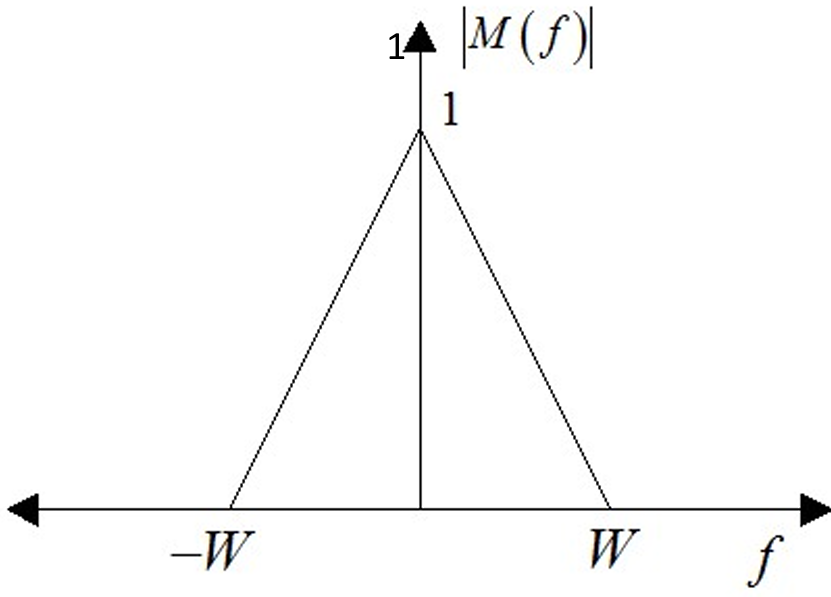
\includegraphics[width=0.5\textwidth]{imagenes/Parte_1/Actividad_1/fig1.png}
    \caption{Espectro de la señal de mensaje $m(t)$}
    \label{fig:1}
\end{figure}

\subsection*{El ancho de banda de la señal es de 1000 Hz, y es aplicada a un modulador producto con portadora $A\cos(2\pi f t)$. La señal modulada $s(t)$ es luego aplicada a un Detector Coherente como el indicado en la Fig. 2 del Ejercicio 4.}  


\subsection*{a) Graficar el espectro obtenido en la salida del detector para $f_c=500$ Hz. ¿Se recibe la señal enviada? Justifique.} 


Al aplicar el detector coherente en la señal $m(t)$ se obtiene lo siguiente:
\bigskip

La señal $m(t)$ (el mensaje) se multiplica con la portadora en el tiempo o se convoluciona en frecuencia con la finalidad de obtener $s(t)$.
\bigskip

La señal en el dominio del tiempo es:

\[
s(t) = A_c \, m(t) \cos(2\pi f_c t)
\]

En el dominio de la frecuencia:

\[
S(f) = \frac{A_c}{2} \left[ M(f-f_c) + M(f+f_c) \right]
\]

Reemplazando por valores numéricos:
\[
S(f) = \frac{A_c}{2} \left[ M(f-500) + M(f+500) \right]
\]

en la Fig. \ref{fig:1a_solapamiento} se muestra el espectro centrado en $\pm 500 [Hz]$

    \begin{figure}[H]
        \centering
        \includegraphics[width=0.5\linewidth]{imagenes/Parte_1/Actividad_1/señal_solapada.jpg}
        \caption{Solapamiento.}
        \label{fig:1a_solapamiento}
    \end{figure}
    
Luego, al multiplicar por el oscilador local y aplicando la propiedad trigonométrica del producto de cosenos $\cos\alpha \cos\beta = \tfrac{1}{2}\left[\cos(\alpha+\beta)+\cos(\alpha-\beta)\right]$, se obtiene:

\[
v(t) = s(t) \cdot \frac{A'_c}{2} \cos(2\pi f_c t) =  \frac{A'_c A_c}{2} \, m(t) \Big[ \cos\big(2\pi(f_c-f_c)t + \phi \big)  + \cos\big(2\pi(f_c+f_c)t\big) \Big]
\]
\[
 = \frac{A'_c A_c}{2} \, m(t) \Big[\cos\big(\phi \big)  + \cos\big(2\pi2(f_c)t\big) \Big] 
\]

En el dominio de la frecuencia:

\[
V(f) = \frac{A'_c A_c}{2}\cos(\phi)\, M(f) \;+\; \frac{A'_c A_c}{4}\Big[ M(f-2f_c) + M(f+2f_c) \Big]
\]

Reemplazando por valores numéricos: 
\[
V(f) = \frac{A'_c A_c}{2}\cos(\phi)\, M(f) \;+\; \frac{A'_c A_c}{4}\Big[ M(f-1000) + M(f+1000) \Big]
\]

Por ultimo, la señal pasa por el filtro pasa bajas y se obtiene la siguiente salida:

\[
v_o(t) = \frac{A'_c A_c}{2}\cos(\phi)\, m(t) 
\]

En el dominio de la frecuencia:
\[
V_o(f) = \frac{A'_c A_c}{2}\cos(\phi)\, M(f) 
\]

En la  Fig.~\ref{fig:señal_reconstruida_solapada} se observa que el espectro obtenido a la salida del detector para $f_c=500 Hz$ y con $\phi = 0$ no se recibe la señal enviada, debido a que la frecuencia de la portadora no es como mínimo dos veces mayor que la frecuencia máxima de la señal y con la amplitud a la mitad.

\begin{figure}
    \centering
    \includegraphics[width=0.5\linewidth]{imagenes/Parte_1/Actividad_1/señal_reconstruida_solapada.jpg}
    \caption{Señal reconstruida.}
    \label{fig:señal_reconstruida_solapada}
\end{figure}
    
\subsection*{b) Repetir para $f_c=10$ kHz.}  

Al aplicar el detector coherente en la señal m(t) pero esta vez con una frecuencia de portadora $f_c=10$ kHz y se obtiene lo siguiente:
\bigskip

La señal m(t) (el mensaje) se multiplica con la portadora en el tiempo o se convoluciona en frecuencia con la finalidad de obtener s(t).
\bigskip

La señal en el dominio del tiempo es:

\[
s(t) = A_c \, m(t) \cos(2\pi f_c t)
\]

En el dominio de la frecuencia:

\[
S(f) = \frac{A_c}{2} \left[ M(f-f_c) + M(f+f_c) \right]
\]

Reemplazando por valores numéricos:
\[
S(f) = \frac{A_c}{2} \left[ M(f-10000) + M(f+10000) \right]
\]

Luego, al multiplicar por el oscilador local y aplicando la propiedad trigonométrica del producto de cosenos $\cos\alpha \cos\beta = \tfrac{1}{2}\left[\cos(\alpha+\beta)+\cos(\alpha-\beta)\right]$, se obtiene $v(t)$:

\[
v(t) = s(t) \cdot \frac{A'_c}{2} \cos(2\pi f_c t) =  \frac{A'_c A_c}{2} \, m(t) \Big[ \cos\big(2\pi(f_c-f_c)t + \phi \big)  + \cos\big(2\pi(f_c+f_c)t\big) \Big]
\]
\[
 = \frac{A'_c A_c}{2} \, m(t) \Big[\cos\big(\phi \big)  + \cos\big(2\pi2(f_c)t\big) \Big] 
\]

En el dominio de la frecuencia:

\[
V(f) = \frac{A'_c A_c}{2}\cos(\phi)\, M(f) \;+\; \frac{A'_c A_c}{4}\Big[ M(f-2f_c) + M(f+2f_c) \Big]
\]

Reemplazando por valores numéricos: 

\[
V(f) = \frac{A'_c A_c}{2}\cos(\phi)\, M(f) \;+\; \frac{A'_c A_c}{4}\Big[ M(f-20000) + M(f+20000) \Big]
\]

Por ultimo, la señal pasa por el filtro pasa bajas y se obtiene la siguiente salida:

\[
v_o(t) = \frac{A'_c A_c}{2}\cos(\phi)\, m(t) 
\]

En el dominio de la frecuencia:
\[
V_o(f) = \frac{A'_c A_c}{2}\cos(\phi)\, M(f) 
\]


Al aplicar los pasos anteriores pero con una frecuencia de portadora que es mucho mayor a la frecuencia máxima de la señal y con $\phi = 0$, se observa en la Fig.~\ref{fig:señal_reconstruida_perfecta} que no hay solapamiento y a la salida la señal del mensaje es la misma pero con la amplitud a la mitad.

    \begin{figure}[H]
        \centering
        \includegraphics[width=0.5\linewidth]{imagenes/Parte_1/Actividad_1/señal_reconstruida_perfecta.jpg}
        \caption{Señal reconstruida.}
        \label{fig:señal_reconstruida_perfecta}
    \end{figure}
        

\subsection*{c) Determinar la mínima frecuencia de portadora necesaria para recuperar $m(t)$ sin distorsión.}  


    Para recuperar $m(t)$ sin distorsión mediante un detector de envolvente (o en general para evitar solapamiento espectral entre bandas), la portadora debe cumplir
    \[
    f_c>f_{\max},
    \]
    siendo $f_{\max}$ la máxima componente de frecuencia presente en $m(t)$. En la práctica se recomienda $f_c\gg f_{\max}$ para asegurar una buena separación entre la portadora y la variación de la envolvente y para facilitar el filtrado.

    
